\chapter{deSolve}
\section{Introduction to Computational Differential Solutions}

Many of the systems studied in life sciences, environmental sciences, and physical sciences can be modeled with differential equations. Differential equations serve to model rates of change, which are often easier to measure than every interaction in the system. A differential equation is an equation for a function that relates the values of the function to the values of its derivatives. An ordinary differential equation (ODE) is a differential equation for a function of a single variable (such as $x(t)$), while a partial differential equation (PDE) is a differential equation for a function of several variables (such as $v(x,y,z,t)$). An ODE contains ordinary derivatives and a PDE contains partial derivatives. Typically, PDE's are much harder to solve than ODE's \cite{chasnov}. \\

Initial Value Problems (IVPs) involve differential equations where certain initial values in the model are known. The \texttt{deSolve} package uses computational means to analyze and compute the values of states in such models. In a differential equation, the state is the variable that is varied with respect to the independent variable in the system. Parameters, on the other hand, are values that signify some characteristic or attribute of the system. For example, in the given system of equations:

\begin{gather*}
    \frac{dY}{dt}=aY
\end{gather*}

The state of the differential equation is $Y$. The independent variable in this system is $t$. Finally, $a$ is a parameter that can be varied to vary the solution. In this lab, we will analyze systems of ordinary first-order differential equations, which relate the first derivative to states and parameters.

\subsection{Examples of Differential Equations}

The \textit{Malthusian law of population growth} is used to model the populations of certain kinds of organisms living in ideal environments for limited lengths of time $t$. It gives the rate at which a population $p$ changes with respect to $t$. The value of the constant $r$ depends on the organism.

\begin{gather*}
    \frac{dp}{dt}=rp
\end{gather*}

This \textit{second-order reaction rate} law gives the rate at which a single chemical species combines to produce a new species, such as methyl radicals combining in a gas to form ethane molecules.

\begin{gather*}
    \frac{dx}{dt}=k(A-x)^2
\end{gather*}

This equation models the motion of a damped mass-spring system subjected to a time-dependent force $F(t)$.

\begin{gather*}
    m\frac{d^2 x}{dt^2}+b\frac{dx}{dt}+kx=F(t)
\end{gather*}

\section{Installation}

To install the \texttt{deSolve} package in R, enter the following code into the command line. Installation may produce warnings that are generally inconsequential to the overall usage of the package. However, if the package does not install correctly, contact the package developers.

\begin{figure}[H]
\centering
\caption{Installation}
\begin{lstlisting}
 > install.packages(``deSolve'')
 > library(deSolve)
\end{lstlisting}
\end{figure}

\section{Objectives of Case Study}

There are certain objectives that students should focus to accomplish while completing this activity. 

\subsection{Objective 1}
\textbf{Objective: } Know what ordinary differential equations and partial differential equations are. For the case studies that follow, it is inconsequential for students to understand the structure and function of ordinary differential equations.

\subsection{Objective 2}
\textbf{Objective: } Understand how initial value problems arise in ordinary differential equation systems in the natural sciences. That is, use initial values found in nature and differential equation models to produce valid solutions.

\subsection{Objective 3}
\textbf{Objective: } Know how to set up a differential equation given a system and the relationship between rates. This is important for modeling a given system.

\subsection{Objective 4}
\textbf{Objective: } Know how to use \texttt{deSolve} to computationally solve systems of ordinary first-order differential equations. This R package allows for computational solutions that effectively model the changes in the dependent variables of the system.

\section{Case Study - Dampened Mass-Spring System}

As discussed in the examples section, a well-known second-order differential equation is used to analyze the motion of an oscillating mass-spring. 

\begin{figure}[H]
    \centering
    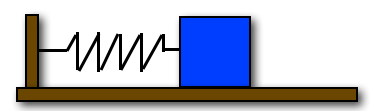
\includegraphics[width=15cm]{pictures-diffeq/mass-spring.jpeg}
    \caption{A mass-spring system}
\end{figure}

A mass-spring system is often called a harmonic oscillator. In an idealized system where no heat loss occurs, the mass-spring oscillator will continue oscillating forever. \\

The nature of a spring can be described using a single parameter, often noted as $k$. The spring constant $k$ is used primarily in Hooke's Law, which relates the amount a spring stretches from rest, $x$, to the amount of force $F$ that is applied on the mass $m$. Hooke's Law states that:

\begin{gather*}
    F=-kx
\end{gather*}

By Newton's Second Law, we also know that:

\begin{gather*}
    F=m\frac{d^2 x}{dt^2}
\end{gather*}

Therefore, we can create a second-order differential equation for the idealized mass-spring oscillator:

\begin{gather*}
    m\frac{d^2 x}{dt^2}=-kx\\
    \boxed{m\frac{d^2 x}{dt^2}+kx=0}
\end{gather*}

Unfortunately, due to the complexity of behaviors and solutions in second-order differential equations, it is computationally easier to create a system of differential equations $x_1', x_2', \hdots, x_n'$ that model the system. \\

We begin with a few basic states that will represent the differential equations in our system.

\begin{gather*}
    x_1 = x\\
    x_2 = \frac{dx}{dt}
\end{gather*}

We compute the derivatives of these states:

\begin{gather*}
    x_1' = x' = x_2\\
    x_2' = x''
\end{gather*}

By solving the second-order differential equation in terms of the second derivative $x''$:

\begin{gather*}
    m\frac{d^2 x}{dt^2}+kx=0\\
    mx''+kx=0\\
    x''=-\frac{k}{m}x=-\frac{k}{m}x_1
\end{gather*}

Therefore, the system of ordinary first-order differential equations that we are trying to solve is:

\begin{gather*}
    \frac{dx_1}{dt}=x_2\\
    \frac{dx_2}{dt}=-\frac{k}{m}x_1
\end{gather*}

\subsection{Computational Solutions}

We begin by setting up the environment to begin using the \texttt{deSolve} package. We import the library and clear the environment variables.\\

\begin{lstlisting}
# Author:       First Last
# Date:         Month Date Year
# Name:         DiffEq.R

# Import the library into R
library(deSolve)

# Clear variables from environment
rm(list = ls())
\end{lstlisting}

As stated in the introduction, we are solving an initial value problem. In this case, we use arbitrary values for states and parameters. We initialize $x_1=100$ to suggest that the spring is stretched 100 meters past it's rest phase. Furthermore, $x_2=0$ to suggest that the motion begins from rest, when the rate of change is 0.\\

\begin{lstlisting}
# m is the mass of the object (1 kg)
# k is the spring constant (50 kg / s^2)
parameters <- c(m = 1, k = 50)

# X is the first differential equation (100 m)
# Y is the second differential equation (0 m/s)
state <- c(X = 100, Y = 0)
\end{lstlisting}

We can define a function that represents the system of differential equations we have defined. Such a function will effectively relate the state and parameters to the derivatives in question. 

\begin{lstlisting}
# Function that defines the system
system <- function(t, state, parameters) {
    with(as.list(c(state, parameters)), {
        dX <- Y
        dY <- -1*(k/m)X
        
        list(c(dX, dY))
    })
}
\end{lstlisting}

We run the simulation over a certain time interval with discreet differences between every time value. Finally, we run the \texttt{ode()} function to produce the discreet values.\\

\begin{lstlisting}
# The sequence of time run in the simulation
times <- seq(0, 10, by=0.01)

# Generate curves that are solutions to the system of differential equations
out <- ode(y=state, times=times,func=system, parms=parameters)
\end{lstlisting}

Running the command above will generate data that is stored in \texttt{out}. We can plot this data out. From our derivation, we know that the value of $x_1=x$. Therefore, the solution to $x_1$ is equal to the solution of the second-order differential equation. We also plot how the two variables, $x_1$ and $x_2$, vary in comparison to each other. We plot the following:\\

\begin{lstlisting}
plot(out[,"time"], out[,"X"], xlab="time", ylab="displacement", pch=19)
plot(out[,"X"], out[,"Y"], xlab="displacement", ylab="velocity", pch=19)
\end{lstlisting}

\begin{figure}[H]
    \centering
    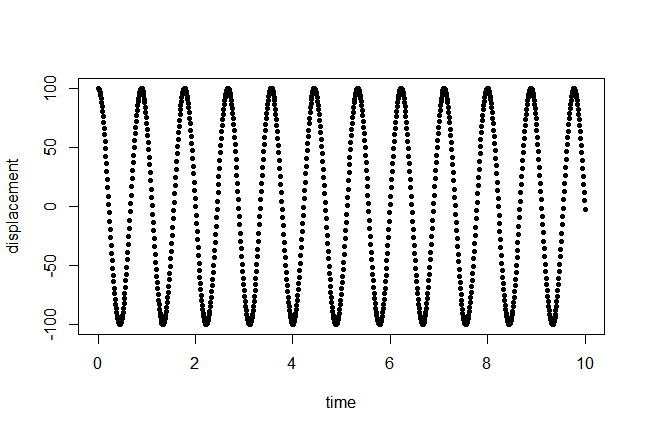
\includegraphics[width=12cm]{pictures-diffeq/plot1.png}
    \caption{The displacement of the spring over time}
\end{figure}

\begin{figure}[H]
    \centering
    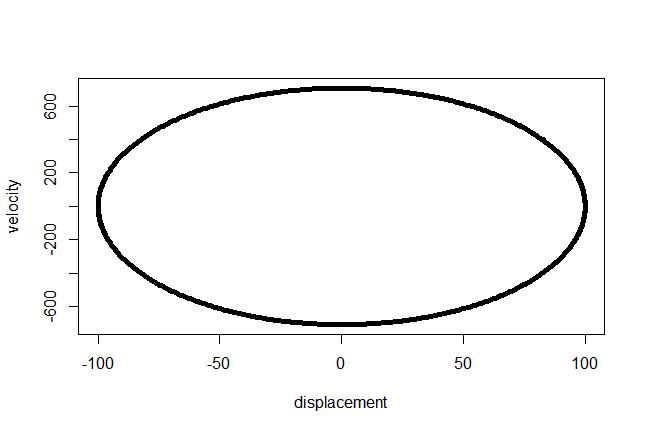
\includegraphics[width=12cm]{pictures-diffeq/plot2.png}
    \caption{The relationship between $x_1$ and $x_2$}
\end{figure}

\subsection{Improving the System}

However, this idealized system does not capture the motion of a spring that is dampened by other factors, such as heat loss by friction. Such a system is known as a \textbf{Dampened Mass-Spring Oscillator}. The spring looses momentum with relation to its velocity, which is the derivative of the position $x$. Therefore, we can add a new parameter to the second-order differential equation, $b$, that accounts for the dampening of the motion of the spring.

\begin{gather*}
    m\frac{d^2 x}{dt^2}+b\frac{dx}{dt}+kx=0
\end{gather*}

Using the method described above to convert the second-order differential equation into a system of first-order differential equations, we get:

\begin{gather*}
\frac{dx_1}{dt}=x_2\\
\frac{dx_2}{dt}=-\frac{k}{m}x_1 - \frac{b}{m}x_2
\end{gather*}

We modify our systems function in R to account for the velocity-dependent dampening of the spring as follows:

\begin{lstlisting}
# m is the mass of the object (1 kg)
# b is the dampening of the object (0.25)
# k is the spring constant (50 kg / s^2)
parameters <- c(m = 1, b = 0.25, k = 50)

# Function that defines the system
system <- function(t, state, parameters) {
    with(as.list(c(state, parameters)), {
        dX <- Y
        dY <- -1*(k/m)X - (b/m)Y
    })
}
\end{lstlisting}

Running the simulation again, we get the following graphs. Notice that the range of the motion of the spring-mass system continually decreases as time passes. This accounts for much of the heat loss that a dampened spring experiences. 

\begin{figure}[H]
    \centering
    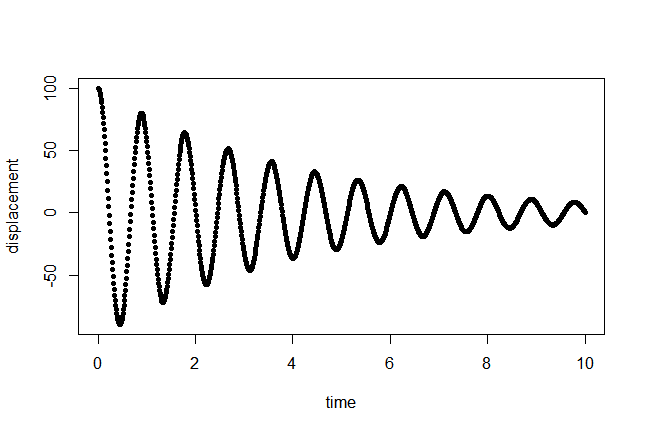
\includegraphics[width=12cm]{pictures-diffeq/plot3.png}
    \caption{The displacement of the spring over time}
\end{figure}

\begin{figure}[H]
    \centering
    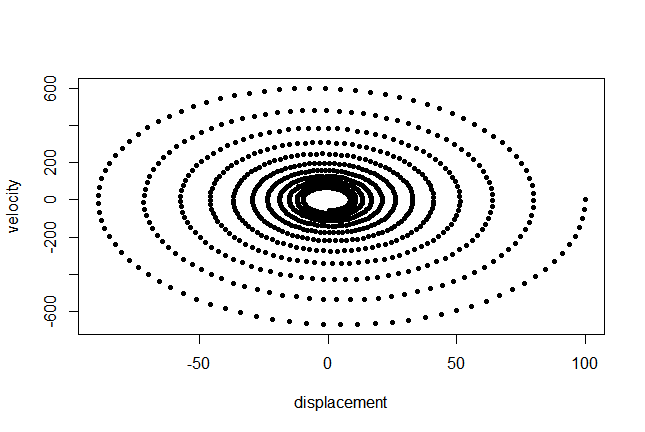
\includegraphics[width=12cm]{pictures-diffeq/plot4.png}
    \caption{The relationship between $x_1$ and $x_2$}
\end{figure}

\section{Student Assignment - Modelling of Genetic Processes}

Many of the genetic processes that are studied in the field of molecular biology can be modeled using systems of differential equations. The student is tasked with understanding many of theses systems and modeling them. It is important for us to go over the \textit{central dogma of molecular biology} before proceeding any further.\\

The three main components of this dogma are DNA, mRNA, and proteins. Proteins are generally the effectors in our cells, responsible for life-critical tasks, enzymatic processes, and regulation. Every protein has its own function and specificity. Ribosomal subunits, responsible for synthesizing proteins, get instructions for synthesis from polymer strands made of nucleotides known as mRNA. mRNA strands, in turn, are synthesized using instructions from another polymer known as DNA, which is the only heritable molecule present in the cell (as long as we ignore mitochondrial DNA that is passed down from a maternal lineage). We will also quickly review the processes of transcription and translation in depth. However, a strong foundation in biology is not necessary for modelling the problems that will follow. \\

\begin{itemize}
    \item \textbf{Transcription: } Transcription is the process by which the information contained in a section of DNA (most often a gene) is transferred to a newly assembled piece of messenger RNA (mRNA). Transcription is triggered by the binding of RNA Polymerase to specific regions on the DNA called promoters, and is enabled/facilitated or impeded by a range fo promoter-specific proteins called transcription factors \cite{stan}.
    \item \textbf{Translation: } During translation, proteins are produced by ribosomes that bind to a specific site of the mRNA (the ribosome binding site - RBS) and then move along the mRNA chain converting triplets of bases or ``codons'' on the mRNA into the appropriate peptide chain of amino acids defining the desired protein. The mRNA is read by the ribosome as triplet of bases, usually beginning with an AUG, or an initiator methionine codon downstream of the ribosome binding site. Complexes of initiation factors and elongation factors bring aminoacylated transfer RNAs (tRNAs) into the riboosome-mRNA complex, matching the codon in the mRNA to the anti-codon in the tRNA, thereby adding the correct amino acid in the growing peptide sequence encoding the emerging protein. As the amino acids are linked together into the growing peptide chain, they begin folding into the correct conformation. This folding continues until the nascent polypeptide chain is released from the ribosome as a mature protein \cite{stan}.
\end{itemize}

\begin{figure}[H]
    \centering
    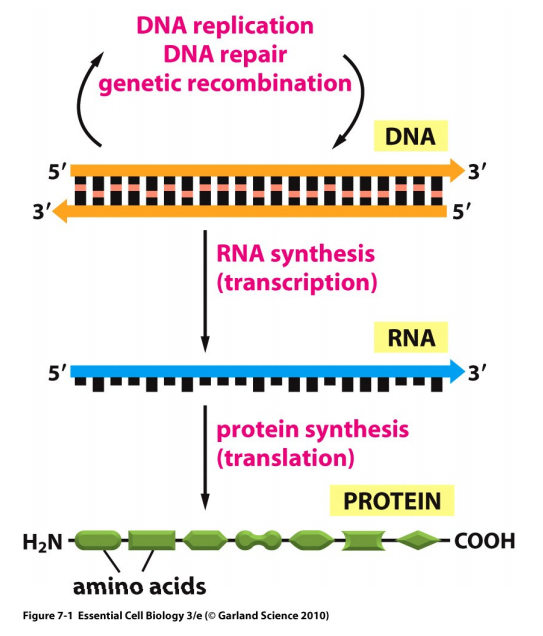
\includegraphics[width=10cm]{pictures-diffeq/img1.png}
    \caption{The Central Dogma of Molecular Biology}
\end{figure}

\subsection{Constitutive Gene Expression}

\textbf{Problem Statement: } Model the system of constitutive gene expression in terms of the central dogma of molecular biology, mRNA degradation, and protein degradation.\\

Constitutive gene expression is the process that occurs when a gene is always on. That is, the gene is not regulated in any manner and simply follows the central dogma of biology. In such a case, we have to consider a few rates that occur in the system. 

\begin{itemize}
    \item $\frac{dm}{dt}$ is the rate at which mRNA is synthesized from DNA. It will be one of the differential equations students will use in their system.
    \item $\frac{dp}{dt}$ is the rate at which the protein in question is synthesized from DNA. It will be the other differential equation students will consider in their system.
    \item $k_{m}$ is the constitutive transcription rate. It is considered to be constant, and it represents the number of mRNA molecules produced per gene, per unit of time. We assume that there is only one copy of the gene in the cell. In the case of bacterial cells, where plasmid-located genes occur in multiple copies in different plasmids, we would multiply the rate $k_1$ by the number of copies $N$ in the cell to obtain a proper rate.
    \item $k_{p}$ is the translation rate. It is considered to be constant, and it represents the number or protein molecules produced per mRNA molecule, per unit of time.
    \item $d_{m}$ is the mRNA degradation rate, measured as the frequency at which mRNA molecules degrade.
    \item $d_{p}$ is the protein degradation rate, measured as the frequency at which protein molecules degrade.
\end{itemize}

\noindent \textbf{Sample Student Solution} \\

The student should be capable of modeling the system using the rates provided above. The system we are considering should account for transcription, translation, and the degradation of components in the process.

\begin{figure}[H]
    \centering
    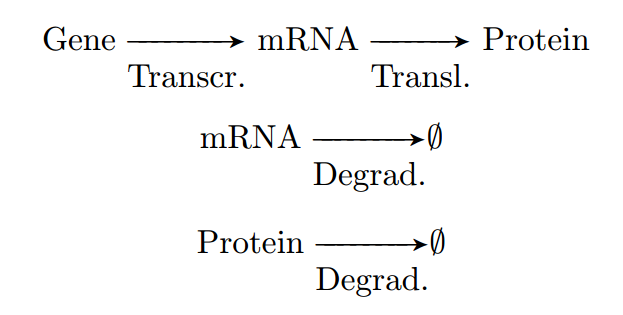
\includegraphics[width=8cm]{pictures-diffeq/img2.png}
    \caption{The constitutive gene expression system}
\end{figure}

The rate at which mRNA is transcribed is equal to the rate provided to us, $k_{m}$. Furthermore, we account for the rate of degradation by multiplying the frequency rate $d_{m}$ by the number of mRNA molecules in the system. The rate at which protein molecules are translated is equal to the rate $k_{p}$. Similar to the mRNA system, the degradation occurs as a product of $d_{p}$ and the amount of protein produced. 

\begin{gather*}
    \frac{dm}{dt}=k_{m}-d_{m}m\\
    \frac{dp}{dt}=k_{p}m-d_{p}p
\end{gather*}

The student simply has to change certain aspects of the program written by the instructor. In this case, the student must define a new set of states, parameters, and a new system function.

\begin{lstlisting}
library(deSolve)

parameters <- c(km = 10, kp = 5, dm = 1, dp = 3)
state <- c(M = 0, P = 0)

system <- function(t, state, parameters) {
    with(as.list(c(state, parameters)), {
        dM <- km - dm*M
        dP <- dp*M - dp*P
        
        list(c(dM, dP))
    })
}

times <- seq(0, 10, by=0.01)

out <- ode(y = state, times = times, func = system, parms = parameters)

# Plotting Functions
xaxis.range <- range(times)
yaxis.range <- range(min(range(out[,"M"]), range(out[,"P"])), max(range(out[,"M"]), range(out[,"P"])))
plot(out[,"time"], out[,"M"], xlim=xaxis.range, ylim=yaxis.range, col="red", xlab="Time", ylab="Concentration", main="System", pch=19)
points(out[,"time"], out[,"P"], col="blue", pch=19)
legend("bottomright", c("mRNA", "Protein"), pch=c(19, 19), col=c("red", "blue"))
\end{lstlisting}

\begin{figure}[H]
    \centering
    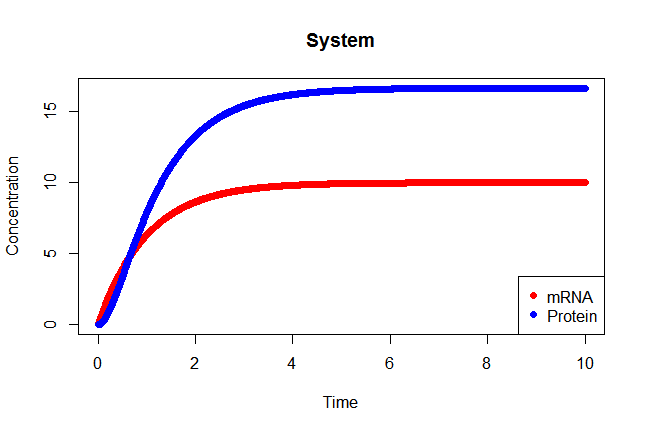
\includegraphics[width=12cm]{pictures-diffeq/plot5.png}
    \caption{Constitutive gene expression concentrations in the system}
\end{figure}

We see that the concentration of proteins and mRNA in the system reaches a steady state with the initial values supplied. It is important for the student to understand that varying the parameters can change the solution to the system. For example, if the rate of degradation of a protein is much larger than the rate at which it is produced, we expect to see no overall protein production. Therefore, it is just as important to choose appropriate initial values as it is to produce a sound differential model. Although arbitrary values are chosen for these samples, students are encouraged to read literature in their field of research or study to find common values for such problems. For instance, the average half life of mRNA in the model system \textit{E. coli} is around 5 minutes. Such information is inconsequential to producing an appropriate model.

\subsection{Gene Transcription Regulation}

Interestingly, most genes that are known today do not follow the constitutive gene expression model. The constant production of proteins can be unnecessary, if not harmful, to  the proper function of the organism. Therefore, multiple layers of regulation occur to ensure that the gene produces proteins at the correct time and the proper rate. There are two major arguments for the necessity of gene regulation in cellular and molecular biology. Firstly, all cells carry the same DNA (and therefore, the same heritable information) but have different developmental stages and functions. Secondly, cells are subject to many environmental perturbations, which can only be dealt with by regulation.\\

Proteins known as transcription factors are generally responsible for the regulation of genes. Transcription factors attach to a region upstream of the gene known as the promoter. The transcription factor can either be an activator (promotes the transcription of the gene) or a repressor (inhibits the transcription of the gene). 

\begin{figure}[H]
    \centering
    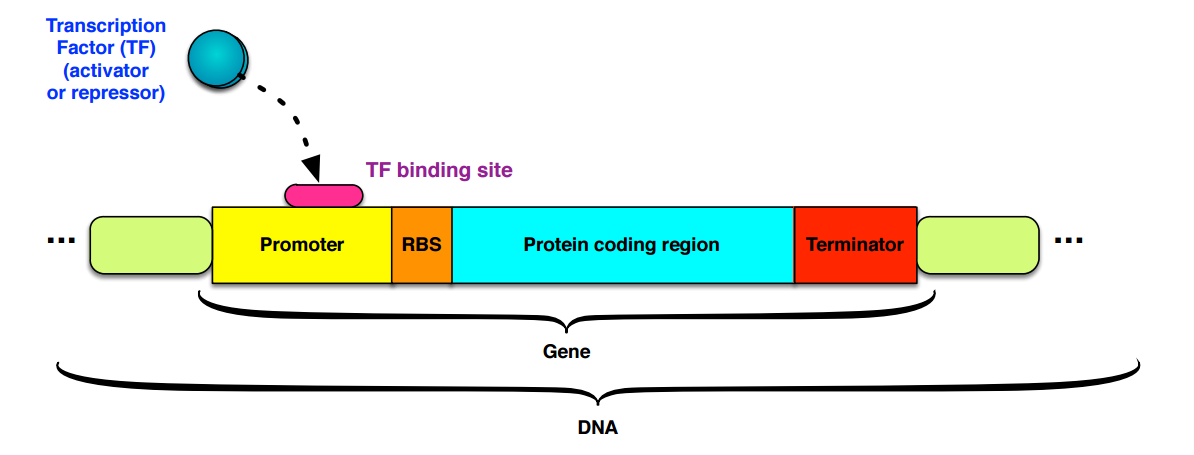
\includegraphics[width=15cm]{pictures-diffeq/img3.png}
    \caption{Action of regulative transcription factors on protein-encodoing DNA regions}
\end{figure}

\subsubsection{Activators and Repressors}

\textbf{Problem Statement: } Model the case of a gene whose transcription is activated by the binding of an activator/repressor to its transcription factor binding site.\\

A gene begins transcription once an activator binds to its corresponding transcription factor binding site. Once activated, the gene goes through the same process that it would during constitutive gene expression. These processes are inhibited once a repressor binds to the transcription factor binding site. This process as a whole is the basis of gene regulation.
Because of the fact that, save for the introduction of activators and repressors, the process that the gene undergoes is identical to constitutive gene expression, many of the rates from the constitutive gene expression section are the same in this case. These include $\frac{dm}{dt}$, $\frac{dp}{dt}$, $k_{m}$, $k_{p}$, $d_{m}$, and $d_{p}$. With the introduction of a new parameter (an activator or a repressor), there are subsequently new variables added to this model. The repressor and activator cannot occur at the same time, as the gene can only be activated or inhibited at a certain point in time. These are as follows.

\begin{itemize}
    \item $A$ represents the activator.
    \item $R$ represents the repressor.
    \item $K$ represents the activation or repression coefficient.
    \item $n$ represents the Hill coefficient, or the number of activators/repressors that need to cooperatively bind to the promoter (transcription factor binding site) in order for gene expression to be activated/inhibited.
\end{itemize}

\noindent \textbf{Sample Student Solution} \\

The student should be capable of modeling the system using the rates provided in the constitutive gene expression section, as well as using the new variables provided above. The system we are considering should account for transcription, translation, and the degradation of components in the process.
\begin{figure}[H]
    \centering
    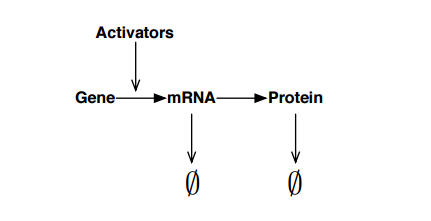
\includegraphics[width=8cm]{pictures-diffeq/activator.png}
    \caption{The activation and subsequent activities of a gene}
\end{figure}
\begin{figure}[H]
    \centering
    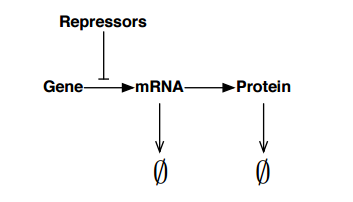
\includegraphics[width=8cm]{pictures-diffeq/Repressors.PNG}
    \caption{The inhibition and subsequent activities of a gene}
\end{figure}

The differential equations used in this model are almost identical to the differential equations used in previous models (the constitutive gene expression model). The only difference is the introduction of the activator/repressor and its coefficients, which is then multiplied by $k_{m}$. 

These are the new differential equations with the introduction of the activator:
\begin{gather*}
    \frac{dm}{dt}=k_{m}\frac{A^{n}}{K^{n}+A^{n}}-d_{m}m\\
    \frac{dp}{dt}=k_{p}m-d_{p}p
\end{gather*}

These are the new differential equations with the introduction of the repressor:
\begin{gather*}
    \frac{dm}{dt}=k_{m}\frac{K^{n}}{K^{n}+R^{n}}-d_{m}m\\
    \frac{dp}{dt}=k_{p}m-d_{p}p
\end{gather*}

As with other cases, the student must define a new set of parameters and system functions in the code. Most of the code remains the same. The following shows the code when using the activator differential equations.

\begin{lstlisting}
library(deSolve)

parameters <- c(km = 10, kp = 5, dm = 4, dp =  4, A = 0.25, K = 0.01, n = 4)
state <- c(M = 0, P = 0)

system <- function(t, state, parameters) {
    with(as.list(c(state, parameters)), {
        dM <- km*(A^n/(K^n+A^n)) - dm*M
        dP <- dp*M - dp*P
        
        list(c(dM, dP))
    })
}
\end{lstlisting}

\begin{figure}[H]
    \centering
    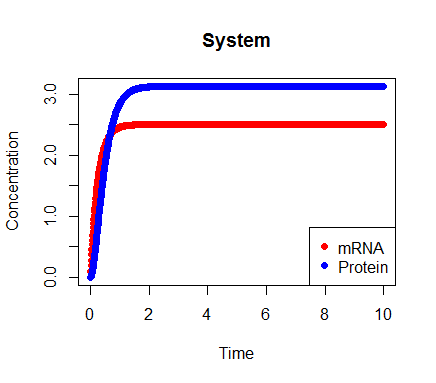
\includegraphics[width=12cm]{pictures-diffeq/activatorplot.png}
    \caption{Gene expression in a system containing activators}
\end{figure}

\subsection{Regulation}

Unfortunately, by simply solving each system individually, it is hard to tell how activation and inhibition affect gene expression models. With the ability to model constitutive gene expression along with activation and regulation, we can compare models where activation and regulation does occur. Using the following values, we can create three concurrent systems and compare them:\\

\begin{lstlisting}
# New parameters in the code
parameters <- c(km = 0.346, kp = 6.931, dm = 0.138, dp = 0.017, A = 200, R = 200, K = 100, n = 2)
state <- c(M = 0, P = 0)

# Constitutive Gene Expression Model
system.const <- function(t, state, parameters) {
    with(as.list(c(state, parameters)), {
        dM <- km - dm*M
        dP <- kp*M - kp*P
        
        list(c(dM, dP))
    }
}

# Activation in Gene Expression
system.act <- function(t, state, parameters) {
    with(as.list(c(state, parameters)), {
        dM <- dm*(A^n / (K^n + A^n)) - dm*M
        dP <- kp*M - dp*P
        
        list(c(dM, dP))
    })
}

# Inhibition in Gene Expression
system.rep <- function(t, state, parameters) {
    with(as.list(c(state, parameters)), {
        dM <- kM*(K^n / (K^n + R^n)) - dm*M
        dP <- kp*M - dp*P
        
        list(c(dM, dP))
    })
}

# Independent variable
times <- seq(0, 400, by=1)

# Computing the solution to all three models
out.const <- ode(y = state, times = times, func = system.const, parms = parameters)
out.act <- ode(y = state, times = times, func = system.act, parms = parameters)
out.rep <- ode(y = state, times = times, func = system.rep, parms = parameters)

# Plotting functions
plot(out.const[,"time"], out.const[,"P"], col="red", xlab="Time", ylab="Concentration", main="System", pch=19)
points(out.act[,"time"], out.act[,"P"], col="green", pch=19)
points(out.rep[,"time"], out.rep[,"P"], col="yellow", pch=19)
legend("bottomright", c("Protein CONST", "Protein ACT", "Protein REP"), pch=c(19, 19, 19), col=c("red", "green", "yellow"))
\end{lstlisting}

The code will produce the following graphics. Notice that the constitutive protein expression runs unaffected. The activation gene expression curve takes longer to achieve expression because it takes time for activators to act as transcription factors before transcription can take place. Furthermore, the repressed curve is much lower than both, as is expected from such systems.

\begin{figure}[H]
    \centering
    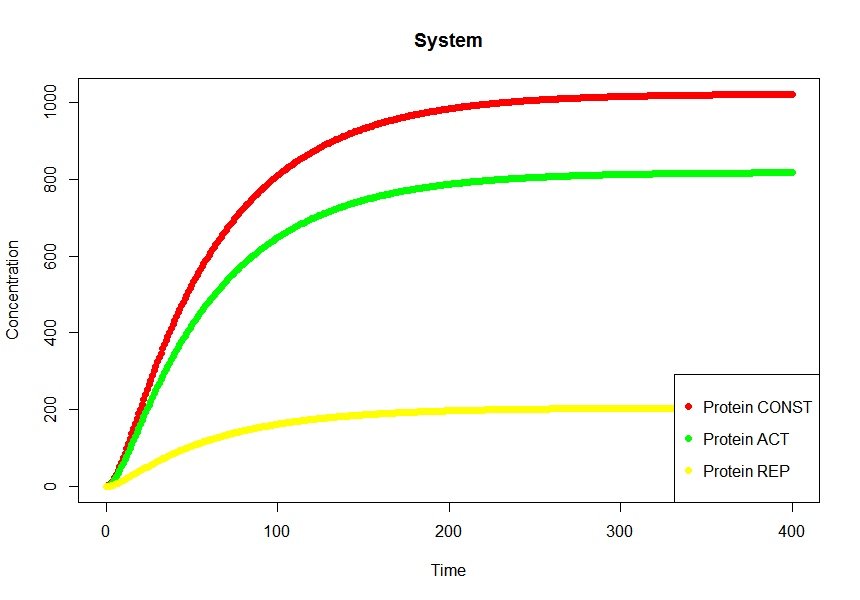
\includegraphics[width=14cm]{pictures-diffeq/plot6.png}
    \caption{Comparing constitutive, activation, and inhibition in gene expression.}
\end{figure}

\section{Conclusion}

Differential equations are used in a variety of different areas to model a wide range of functions, such as the rate that a protein is transcribed or the rate that a population grows. The main function of a differential equation is to model a rate of change. Some of these equations are easily solved by hand, whereas others are more complicated; the \texttt{deSolve} package in R serves to solve and graph a system of differential equation once certain parameters and initial values are entered. Through learning and using \texttt{deSolve}, it is possible to easily solve a system of complex differential equations, as well as view the results graphically and be able to change parameters and values as needed. This streamlines a process of solving equations that occur within all types of science, math, and other processes.

\section{Acknowledgements}

We would like to thank the creators of the \texttt{deSolve} package, Karline Soetaert, Thomas Petzoldt, and R. Woodrow Setzer of the Royal Netherlands Institute of Sea Research. We would also like to thank Mr. Robert Gotwals and the North Carolina School of Science and Mathematics (NCSSM).

\begin{thebibliography}{3}
    \bibitem{soetaert}
        Karline Soetaert, Thomas Petzoldt, and R. Woodrow Setzer. ``Package deSolve: Initial Value Differential Equations in R.'' Royal Netherlands Institute of Sea Research (NIOZ), Yerseke, The Netherlands; Technische Universit{\"a}t, Dresden, Germany; National Center for Computational Toxicology, US Environmental Protection Agency, 2016 (\url{https://cran.r-project.org/web/packages/deSolve/vignettes/deSolve.pdf})
    \bibitem{chasnov}
        Jeffrey R. Chasnov. ``Introduction to Differential Equations.'' Hong Kong University of Science and Technology, 2016 (\url{https://www.math.ust.hk/~machas/differential-equations.pdf})
    \bibitem{stan}
        Dr. Guy-Bart Stan. ``Modelling in Biology,'' Department of Bioengineering, Imperial College of London, 2010 (\url{http://www.bg.ic.ac.uk/research/g.stan/2010_Course_MiB_article.pdf})
\end{thebibliography}

\end{document}
